\section{Study 3: heart rate and accuracy of rPPG measurements}
\label{s:experiment1-study3}

This study presents information regarding the accuracy evaluation of a remote photoplethysmography (rPPG) technique in a gaming context. The technique was applied to estimate the HR of subjects behaving naturally in gaming sessions with induced boredom and stress. Previous work with experiments involving emotions and rPPG were performed under extremely controlled situations with few game-related stimuli. Subjects were not interacting with a complete digital game in any of the experiments, which hindered the accuracy evaluation of rPPG techniques within the context of games research, for instance. Authors commonly used images, videos or text as content to produce the emotional stimuli, in experimental sessions lasting from 20 seconds to 10 minutes.

The aforementioned non-game stimuli content is less likely to produce the reactions of a real gaming session, e.g. spontaneous body movement and facial actions. As opposed to such works, in this study each subject spent an average of 25 minutes in the session, playing three different games that were custom-made to provoke the emotional reactions similar to a natural play session. Subjects were also not instructed regarding how they should move, so body and facial reactions are likely to be the ones the subject would normally perform under a gaming context.

The recordings of game sessions of each subject were divided in video segments of 1 minute each. The rPPG technique by Poh et al. \parencite{poh2011advancements} was applied to each of those video segments to estimate the HR of subjects. An accuracy evaluation of the estimated HR obtained from the video segments was performed in relation to the HR calculated from ground truth.

%In that context, we designed and carried out an experiment focused on the accuracy evaluation of an rPPG technique applied to real gaming sessions, using custom made games as emotion stimuli.  We aim to explore the accuracy of rPPG-estimated HR readings of subjects while playing under such circumstances. To the best of our knowledge, this is the first experiment to measure the accuracy of an rPPG technique with the use of three boredom/stress-inducing games with subjects behaving naturally.

\subsection{Analysis and methods}

Firstly the videos of each game session were divided into several video segments of 60 seconds each, denoted as $V_i$, where $i \in [1, 2, ..., n]$ represents the interval (1 comprehends the time from 0:00 until 1:00, 2 comprehends the time from 1:00 until 2:00, and so on). The use of 60 seconds as the duration of each video segment is based on the work by \textcite{poh2011advancements}.

Since the games have a constantly increasing difficulty level, different subjects might have played the same game for longer or shorter periods of time. As a consequence, the interval $n$ represents the last available interval for each subject and it is likely to be different among subjects. Any remaining video segment of less than 60 seconds was discarded, i.e. if the duration of a game session was not multiple of 60. Following was the calculation of $HR_{gt}(V_i)$, which is the mean HR obtained from the ground truth data of a subject while playing during the video segment $V_i$. It was excluded from the calculation any HR value equal to zero assuming it was a miss-reading.

As previously mentioned in Section \ref{s:literature-rppg-techniques}, the rPPG technique proposed by \textcite{poh2011advancements} is consolidated, extensively mentioned in the literature and presents the best SNR for HR estimation under non-exercising situations. For those reasons, such technique  (refereed as the rPPG technique from now on) was selected to perform the extraction of HR from the video segments. For the comparison, $HR_{video}(V_i)$ was calculated, which is the estimated HR from video segment $V_i$ obtained with the rPPG technique. The evaluation of the accuracy of $HR_{video}$ when compared to $HR_{gt}$ was based on statistical methods used by previous works \parencite{poh2011advancements, rouast2016remote, li2014remote}. The measurement error is calculated as:

\begin{equation}
\label{eqn:hr-error}
HR_{error} = HR_{video} - HR_{gt}
\end{equation}

where $HR_{video}$ is the set of HR estimations by the rPPG technique from the video segments and $HR_{gr}$ is the set of HR means calculated from the ground truth obtained from the watch, as previously described in Section \ref{s:experiment1-study3}. $HR_{error}$ was calculated with video segments of a given game (for the analysis of that game) or with all available segments (for the analysis of all games combined).

The following measurements were also calculated: mean of $HR_{error}$ denoted as $M_e$; standard deviation of $HR_{error}$ denoted as $SD_e$; root mean squared error (RMSE) of $HR_{error}$; mean of error-rate percentage, calculated as:

\begin{equation}
\label{eqn:merate}
M_{eRate} = \frac{1}{N} \sum_{i=1}^{N}\frac{|HR_{error}(V_i)|}{HR_{gt}(V_i)}
\end{equation}

where $V_i$ is a video segment and $N$ is the total of video segments for a given game (or for all games); finally the linear correlation between $HR_{video}$ and $HR_{gt}$ accessed using Pearson's correlation coefficient $r$.

%%%%%%%

The selected rPPG technique was implemented in Matlab R2016a according to the original paper by \textcite{poh2011advancements}. Since the custom algorithm to detect peaks mentioned in the article is unknown, such step was replaced by the identification of the highest peak in the frequency domain after an FFT operation. This operation is commonly used in the HR estimation phase of rPPG techniques, as explained in Section \ref{s:literature-rppg-structure}.

The implementation of the rPPG technique was validated with a procedure similar to the one described by \textcite{li2014remote}. Firstly a manual inspection of all video recordings from the experiment was performed and a segment $V'_i$ of 30 seconds (1500 frames) was exerted from each video where the subject presented the least amount of body motion and facial activity. It resulted in a testing set of 20 video segments of 30 seconds each, totalizing 30000 frames of data. The mean HR calculated from ground truth for the testing set was 76.8 bpm (SD 13.4 bpm, min. 55 bpm, max. 110 bpm).

The rPPG technique was then applied to each of those $V'_i$ segments to estimate the HR, evaluating the estimated values using ground truth and the statistical methods previously described. Results are presented in Table \ref{table:rppg-validation}. The numbers indicate the implemented rPGG technique produces accurate and statistically significant results for the estimations, which are aligned with those reported in the original paper. Therefore it is assumed the rPPG technique is correctly implemented and further accuracy measurements obtained during the analysis are due to subject activity, not implementation errors.

\begin{table}
\caption{Performance of the rPPG technique applied to the testing set}
\label{table:rppg-validation}
\centering
\begin{threeparttable}
  \begin{tabular}{ccccc}
  \toprule
    $M_e$ (bpm) & $SD_e$ (bpm) & RMSE (bpm) & $M_{eRate}$ (\%) & $r$ \\
  \midrule
    -0.25 & 1.41 & 1.40 & 1.52 & 0.99* \\
  \bottomrule
  \end{tabular}
  \begin{tablenotes}
    \small
    \item[*]{$p < 0.001$}
  \end{tablenotes}
\end{threeparttable}
\end{table}

\subsection{Results}

The performance of the rPPG technique regarding the extraction of the HR is presented on Table \ref{table:rppg-validation-games}. The first three rows of the table present the performance evaluation calculated with data from each game, while the last row presents the same performance evaluation calculated with data from all games combined. Regarding the analysis of all games combined, the mean estimation error $M_e$ was 2.99 bpm ($SD_e$ 18.83 bpm), RMSE was 19.03 bpm and $M_{eRate}$ was 10.31\%. The low value for $M_e$ suggests feasible overall accuracy of the technique, however the high values for $SD_e$ and $M_{eRate}$ suggest significant variation among the estimations.

As demonstrated by $M_{eRate}$, which is the mean of error-rate percentage, the estimation error of the rPPG technique was equivalent to 10.31\% of the expected HR value calculated from ground truth, on average. On a game level, the mean estimation error $M_e$ was 2.96 bpm ($SD_e$ 19.45 bpm) in the Mushroom game, 0.31 bpm (13.51 bpm) in the Platformer game and 5.18 bpm (21.45 bpm) in the Tetris game. RMSE and $M_{eRate}$ were 19.59 bpm and 10.88\% in the Mushroom game, 13.43 bpm and 7.82\% in the Platformer game, and 21.97 bpm and 11.64\% in the Tetris game, respectively.

All three games presented acceptable values for $M_e$ and significantly higher values for $SD_e$ and $M_{eRate}$, which also suggests feasible results with considerable variations in the estimation error during the analysis of subjects for each game. In particular, the estimations performed during the Platformer game presented the lowest values for $M_e$, RMSE and $M_{eRate}$, which indicates the rPPG technique performed with lower errors and fewer variations among subjects in the Platformer game than it did in the other two games.

\begin{table}
\centering
\caption{Accuracy measurements of the rPPG technique when applied to the video segments of a given game and of all games}
\label{table:rppg-validation-games}
\begin{threeparttable}
  \begin{tabular}{p{0.13\linewidth}ccccc}%
  \toprule
     Game & $M_e$ (bpm) & $SD_e$ (bpm) & RMSE (bpm) & $M_{eRate}$ (\%) & $r$ \\
  \midrule
      Mushroom & 2.96 & 19.45 & 19.59 & 10.88 & 0.45* \\
      Platformer & 0.31 & 13.51 & 13.43 & 7.82 & 0.55* \\
      Tetris & 5.18 & 21.45 & 21.97 & 11.64 & 0.37* \\
      \textit{All} & 2.99 & 18.83 & 19.03 & 10.31 & 0.43* \\
  \bottomrule
  \end{tabular}
  \begin{tablenotes}
    \small
    \item[*]{$p < 0.001$}
  \end{tablenotes}
\end{threeparttable}
\end{table}

The Pearson's correlation coefficient $r$ regarding $HR_{gt}$ (mean HR calculated from the ground truth) and $HR_{video}$ (mean HR estimated via rPPG) is 0.45, 0.55 and 0.37 for the Mushroom, Platformer and Tetris game, respectively. All correlations have statistical significance, $p < 0.001$. The correlation is illustrated in Figure \ref{fig:chart-r-games}. For all three games, there is a positive and medium strength correlation between $HR_{gt}$ and $HR_{video}$, which also indicates the estimations performed by the rPPG technique are feasible. The correlation is stronger in the Platformer game, followed by the Mushroom game and finally by the Tetris game.

\begin{figure}[!h]
\centering
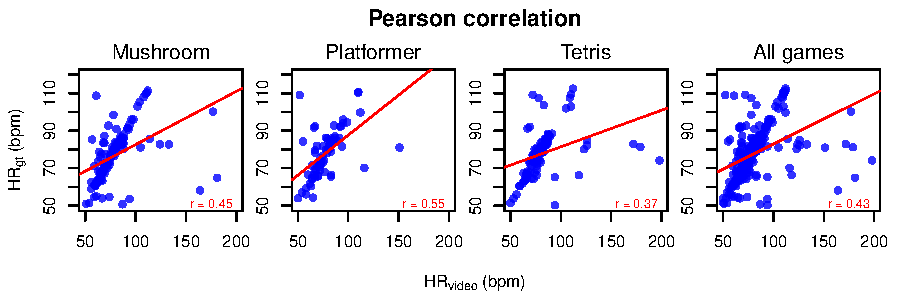
\includegraphics[width=\columnwidth]{Content/figures/correlation-hrgt-hrvideo.pdf}
\caption{Statistical correlation of $HR_{gt}$ and $HR_{video}$ when applied to the video segments of each game, as well as to the video segments of all games.}
\label{fig:chart-r-games}
\end{figure}

To better analyze the variations regarding estimation errors among subjects, figures \ref{fig:chart-hists-me} and \ref{fig:chart-hists} show a distribution of values of $M_e$, RMSE and $M_{eRate}$ for all games combined and individually. The x-axis represents intervals of values of $M_e$, RMSE or $M_{eRate}$ while the y-axis represents the percentage of subjects that presented an estimation error within the interval informed in the x-axis.

Regarding the distribution of values of $M_e$, shown in Figure \ref{fig:chart-hists-me}, overall 66.1\% of the subjects presented estimations with $M_e$ within the interval [-5 bpm, 5 bpm]. For the remaining 33.9\% of the subjects, $M_e$ was spread within the interval [-20 bpm, 35 bpm]. On a game level, $M_e$ was within the interval [-5 bpm, 5 bpm] for 65\%, 68.4\% and 65\% of the subjects of the Mushroom, Platformer and Tetris game, respectively. The values for $M_e$ are more equally distributed for the Platformer game, which explains the lower values of $SD_e$ for that game when compared to the Mushroom and the Tetris game, which present less equally distributed values of $M_e$.

The distribution of values of RMSE, shown in Figure \ref{fig:chart-hists} in the first row, indicate that overall values were lower then 10 bpm for 59.4\% of the subjects, while the remaining of the subjects had RMSE varying from 10 bpm to 50 bpm. On a game level, RMSE was lower than 10 bpm for 50\%, 68.5\% and 60\% of the subjects of the Mushroom, Platformer and Tetris game, respectively.

Regarding $M_{eRate}$, shown in Figure \ref{fig:chart-hists} in the second row, overall 69.5\% of subjects had HR estimations that were up to 10\% different than the expected HR from ground truth. On a game level, in total 73.7\% and 70\% of the estimations performed by the rPPG technique during the Platformer and the Tetris game, respectively, presented $M_{eRate}$ interior or equal to 10\%. Those values are slightly better than the 65\% of the subjects with $M_{eRate}$ up to 10\% in the Mushroom game. Despite the fact that $M_{eRate}$ was similar for both the Platformer and Tetris games, the former presented no subjects whose $M_{eRate}$ was greater than 30\%, while the later presented 10\% of the subjects with $M_{eRate}$ greater than 30\%.

\begin{figure}[!h]
\centering
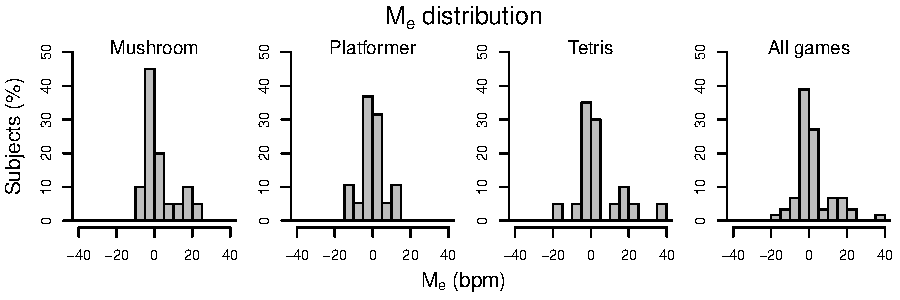
\includegraphics[width=1.0\textwidth]{Content/figures/hist-me.pdf}
\caption{Distribution of values of $M_e$ for all games. The x-axis represents intervals of values of $M_e$ while the y-axis represents the percentage of subjects that presented an estimation error within the interval informed in the x-axis.}
\label{fig:chart-hists-me}
\end{figure}

\begin{figure}[!h]
\centering
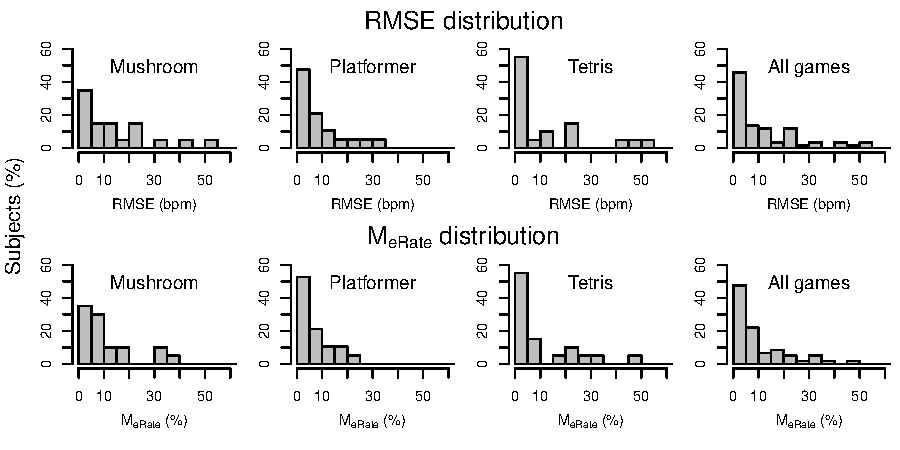
\includegraphics[width=1.0\textwidth]{Content/figures/hist-rmse-mrate.pdf}
\caption{Distribution of values of RMSE and $M_{eRate}$ for all games. The x-axis represents intervals of values of RMSE or $M_{eRate}$ while the y-axis represents the percentage of subjects that presented an estimation error within the interval informed in the x-axis.}
\label{fig:chart-hists}
\end{figure}

\subsection{Discussion}

The results obtained indicate that the use of the selected rPPG technique to estimate HR from videos of gaming sessions is feasible. When the technique was applied to a testing set of 20 manually selected 30 seconds long video segments, whose subject's facial activity and body movement were minimal, the estimations were significantly accurate. As demonstrated by Table \ref{table:rppg-validation}, the mean of error-rate $M_{eRate}$ was 1.52\% and the Pearson's correlation coefficient was $r = 0.99$ for that testing set. Those results were expected since the videos featured an unrealistic condition where subjects remained mostly still with a neutral face.

When the rPPG technique was applied to all gaming sessions, however, body movement and facial activity significantly impacted the estimation performance. It is aligned with previously described works in the literature, which indicate the estimation error increases when subject activities increase \parencite{Wang_2016novel}.

The elevated values for $SD_e$, the standard deviation of $M_e$, suggest significant variations in the estimations among subjects in each video segment. The estimation discrepancies do not seem to be caused by errors equally spread among all gaming sessions, but due to a subset of problematic ones instead. The discrepancies and skewness of the estimations are visible in the scatter plot of the estimated and expected HR values in Figure \ref{fig:chart-r-games}. It shows a cluster of points for each game, however it is surrounded by significantly wrong estimation points. In the Mushroom game, for instance, 5 estimations (bottom right of the chart) were in the interval [120 bpm, 181 bpm] bpm, which is significantly outside the expected ground truth interval of [80 bpm, 110 bpm]. Similar significantly wrong estimations can also be seen in the Platformer and the Tetris game.

The skewed distribution of values of $M_e$, $M_{eRate}$ and RMSE illustrated in figures \ref{fig:chart-hists-me} and \ref{fig:chart-hists} also support that indication. Considering the estimations for all games, in total 69.5\% of them presented $M_{eRate}$ related to an estimation value that was less than 10\% different than the expected HR from ground truth. Additionally 59.4\% of all estimations presented RMSE lower than 10 bpm. That result is slightly worse when compared to similar works that used rPPG techniques and subjects featuring natural movements, whose reported RMSE was between 0.11 and 7.28 bpm.

A direct comparison of the results of this study to the ones of such similar works is unfair however. Despite the fact that the aforementioned works present experiments where subjects are told to behave naturally, their accuracy evaluation is based on artificial human-computer interactions, as previously described in Section \ref{s:experiment1-study3}. The accuracy results of the present study account for body and facial movement caused by games whose focus is entertainment, not artificial interactions. As a consequence, the results are more connected to a scenario involving real and spontaneous reactions to games, showing that the estimations of the rPPG technique are feasible, however skewed by other factors such as natural facial activity and subject movement.

The differences in estimation also seem to be connected to the particularities of each game and subject. Considering the distribution of values of RMSE and $M_{eRate}$, both the Platformer and the Tetris games presented more estimations with lower error than the Mushroom game. The Mushroom game presented 15\% of its estimations with RMSE greater than 30 bpm and $M_{eRate}$ greater than 30\%, which are significantly wrong estimations.

In order to further explore such differences in estimations, the variations of movement and size of the ROI used to track the subject's face along the videos was analyzed. A stable ROI (both in shape and movement) is required for a precise extraction of the plethysmographic signal, so significant variations in the ROI lead to estimation errors. The mean position of the center point of the ROI for each subject in each gaming session was calculated. For each subject in each game session, the Euclidean distance between the center point of the ROI of each frame and the mean center point of the ROI previously calculated (for that subject in that session) was measured.

Similarly the mean length of the ROI diagonal for each subject in each game session was calculated, subtracting it from the length of the ROI diagonal of each frame in that gaming session. Since game sessions differ in time duration, the subject's progress in the game was normalized using the interval [0, 1], where 0 is the start point of the gaming session and 1 its end. Measurements were also subtracted from the sessions mean to facilitate analysis and comparison among different games/subjects.

\begin{figure}[!h]
\centering
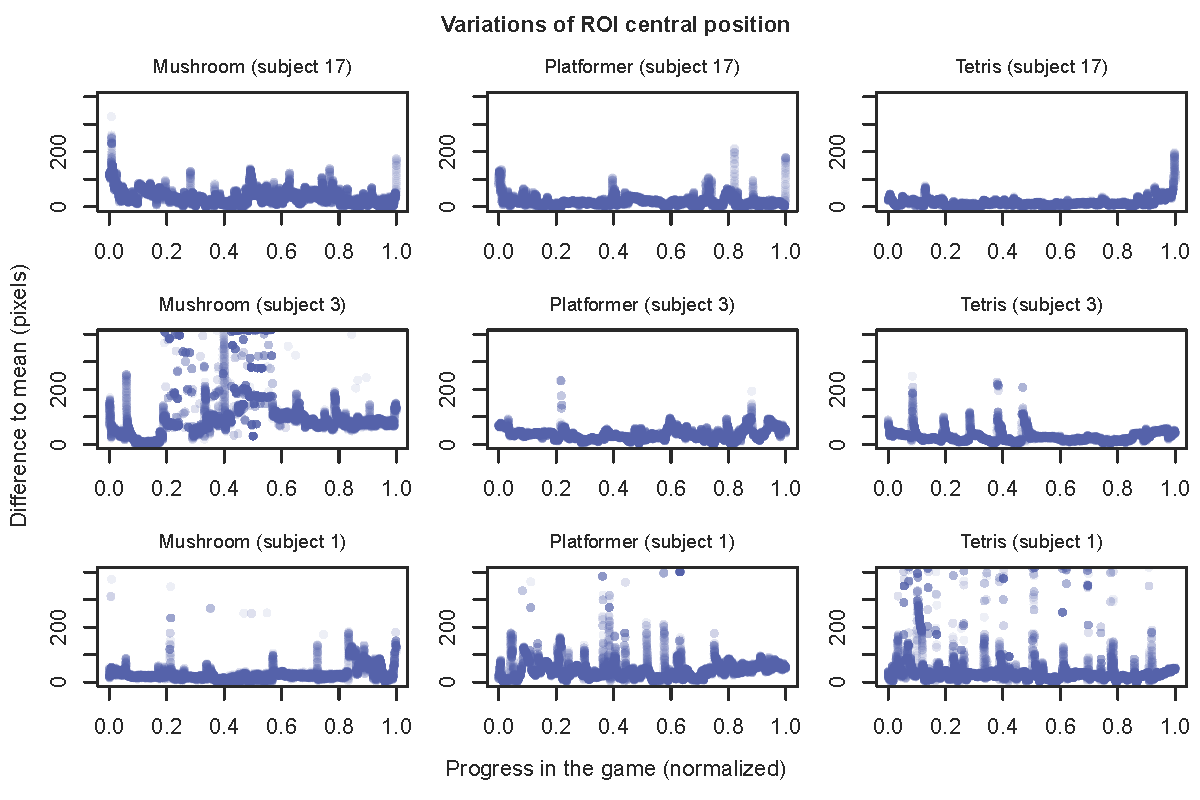
\includegraphics[width=\textwidth]{Content/figures/variation-roi-center.png}
\caption{Variations of distance of the ROI central position for subjects 17 (low estimation errors), 3 (moderate to high estimation errors) and 1 (high estimation errors) during their gaming sessions. Values were subtracted from session mean to facilitate analysis and comparison among different games/subjects.}
\label{fig:chart-roi-anomalies-center}
\end{figure}

Figure \ref{fig:chart-roi-anomalies-center} illustrates some of the patterns observed in the investigation of the distance of the ROI central position. Each row in the figure contains three charts showing the variations of the ROI central position along the gaming sessions of a given subject. The first row contains the investigation of subject 17, who presented, for all his/her gaming sessions combined, -0.33 for $M_e$ ($SD_e$ 1.4) and 1.39 for RMSE (low estimation errors). The second row shows subject 3, who presented 11.47 for $M_e$ ($SD_e$ 16.47) and 19.62 for RMSE (moderate to high estimation errors). Finally the third row shows subject 1, who presented 15.94 for $M_e$ ($SD_e$ 28.5) and 31.96 for RMSE (high estimation errors).

The estimations performed on subject 17 were significantly accurate and the charts regarding the variation of the ROI central position show a stable progression along all gaming sessions. The distance variation (y-axis) remains mostly concentrated within the interval of [0, 100] pixels for all games, which suggest the subject presented few or short movements during gaming sessions. Subject 3 also presented low variation in the Platformer and the Tetris game, however there is a significant variation in the ROI central position in the Mushroom gaming session. The chart indicates significant distance variations of the ROI that are above 200 pixels in a certain period of the game. Finally subject 1 presents high variations in the ROI distance in all gaming sessions, as demonstrated by points above the 200 pixels mark regarding the difference to mean. The Tetris game, in special, present distance variations above 200 pixels during almost the whole session.

\begin{figure}[!h]
\centering
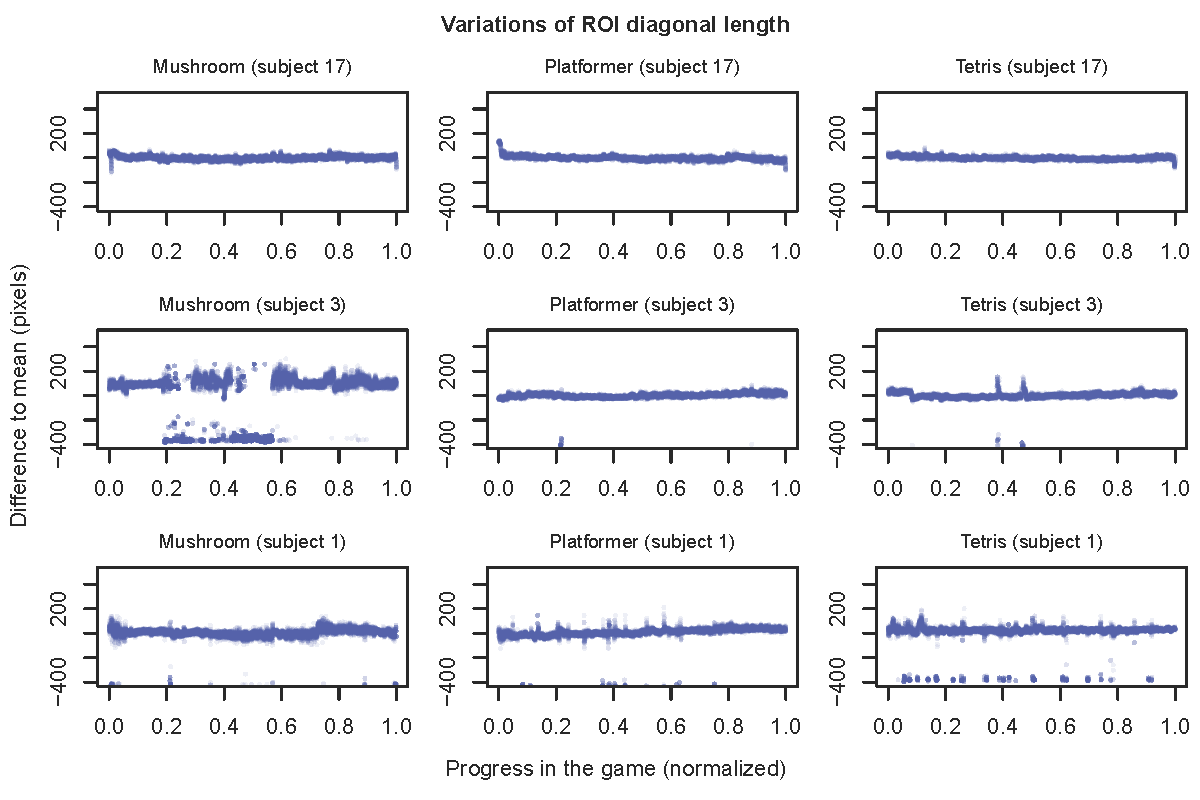
\includegraphics[width=\textwidth]{Content/figures/variation-roi-diagonal.png}
\caption{Variations of ROI diagonal length for subjects 17 (low estimation errors), 3 (moderate to high estimation errors) and 1 (high estimation errors) during their gaming sessions. Values were subtracted from session mean to facilitate analysis and comparison among different games/subjects.}
\label{fig:chart-roi-anomalies-diagonal}
\end{figure}

Figure \ref{fig:chart-roi-anomalies-diagonal} illustrates the same subjects regarding the investigation of the variations of the ROI diagonal length. Similarly to the variations of the ROI central position, the variation of the ROI diagonal length (y-axis) is lower for subject 17 (first row of charts in the figure), since the majority of the values are close to zero. Subject 3 also presents low variations in the ROI diagonal length during the Platformer and the Tetris game, however there are significant changes in the ROI size during a period in the Mushroom game. In such period, the length of the ROI diagonal is negative, i.e. -400 pixels, which indicates the size of the detected ROIs for those frames was smaller than the mean ROI diagonal length. It could be caused by a wrongly detected face (false-negative), for instance. Finally subject 1 presents, to some extent, variations of the ROI diagonal length during the majority of his/her gaming sessions. Those constant variations could be caused by the inability of the face tracking algorithm to stably and continuously detect the subjects face along the frames of the video. The chart shows a distribution of values along the zero mark regarding difference to mean, however they are more spread than those of subject 17, for instance, which indicates higher instability of the ROI size/detection for subject 1. In the Tetris session of subject 1, for instance, there are extreme variation in the ROI diagonal length with values close to -400 pixels, similarly to the ones of subject 3 in the Mushroom game. Such extreme variation could also be explained by a wrongly detected face area during those frames.

An inspection of the videos of subjects with patterns similar to the ones of subjects 3 and 1 revealed sensitive amount of movement and facial activity, including occlusion of the face by the subject's hand, as illustrated by Figure \ref{fig:face-variation}. Any facial occlusion influences the face tracking algorithm used (Viola\&Jones), since it might wrongly detect the face position or do not detect it at all. A flawed face detection step affects the extraction of the plethysmographic signal, because noise is extracted along with the raw signal, making the rPPG technique unable to separate it properly.

Despite the efforts to create games that prevented face occlusion by the subject's hand, such behavior seems to be natural in boring situations. Both Mushroom and Tetris games were more likely to allow players to place a hand in the face to express boredom, since the games could still be played with a single hand when the gameplay speed was not elevated. The Platformer game, on the other hand, is less likely to allow players to use only a single hand to play, which reduced chances of face oclusion inferering with the face tracking algorithm. This could also explain why estimations made during the Platformer game were more accurate than those performed during the other two games. Those extreme cases with facial occlusion are probably affecting the error rates in the analysis, producing less accurate estimations. Such extreme and flawed cases could have removed from the analysis, however the aim is to test how the selected rPPG technique performs in natural gaming situations. A dataset with untreated videos of gaming sessions with natural interactions might produce sub-optimal HR estimations, however it is the understanding that stressing the rPPG technique with less artificial videos provides researchers with insights about possible problems and accuracy limits of such tool.

\begin{figure}
\centering
  \begin{subfigure}[b]{0.5\textwidth}
    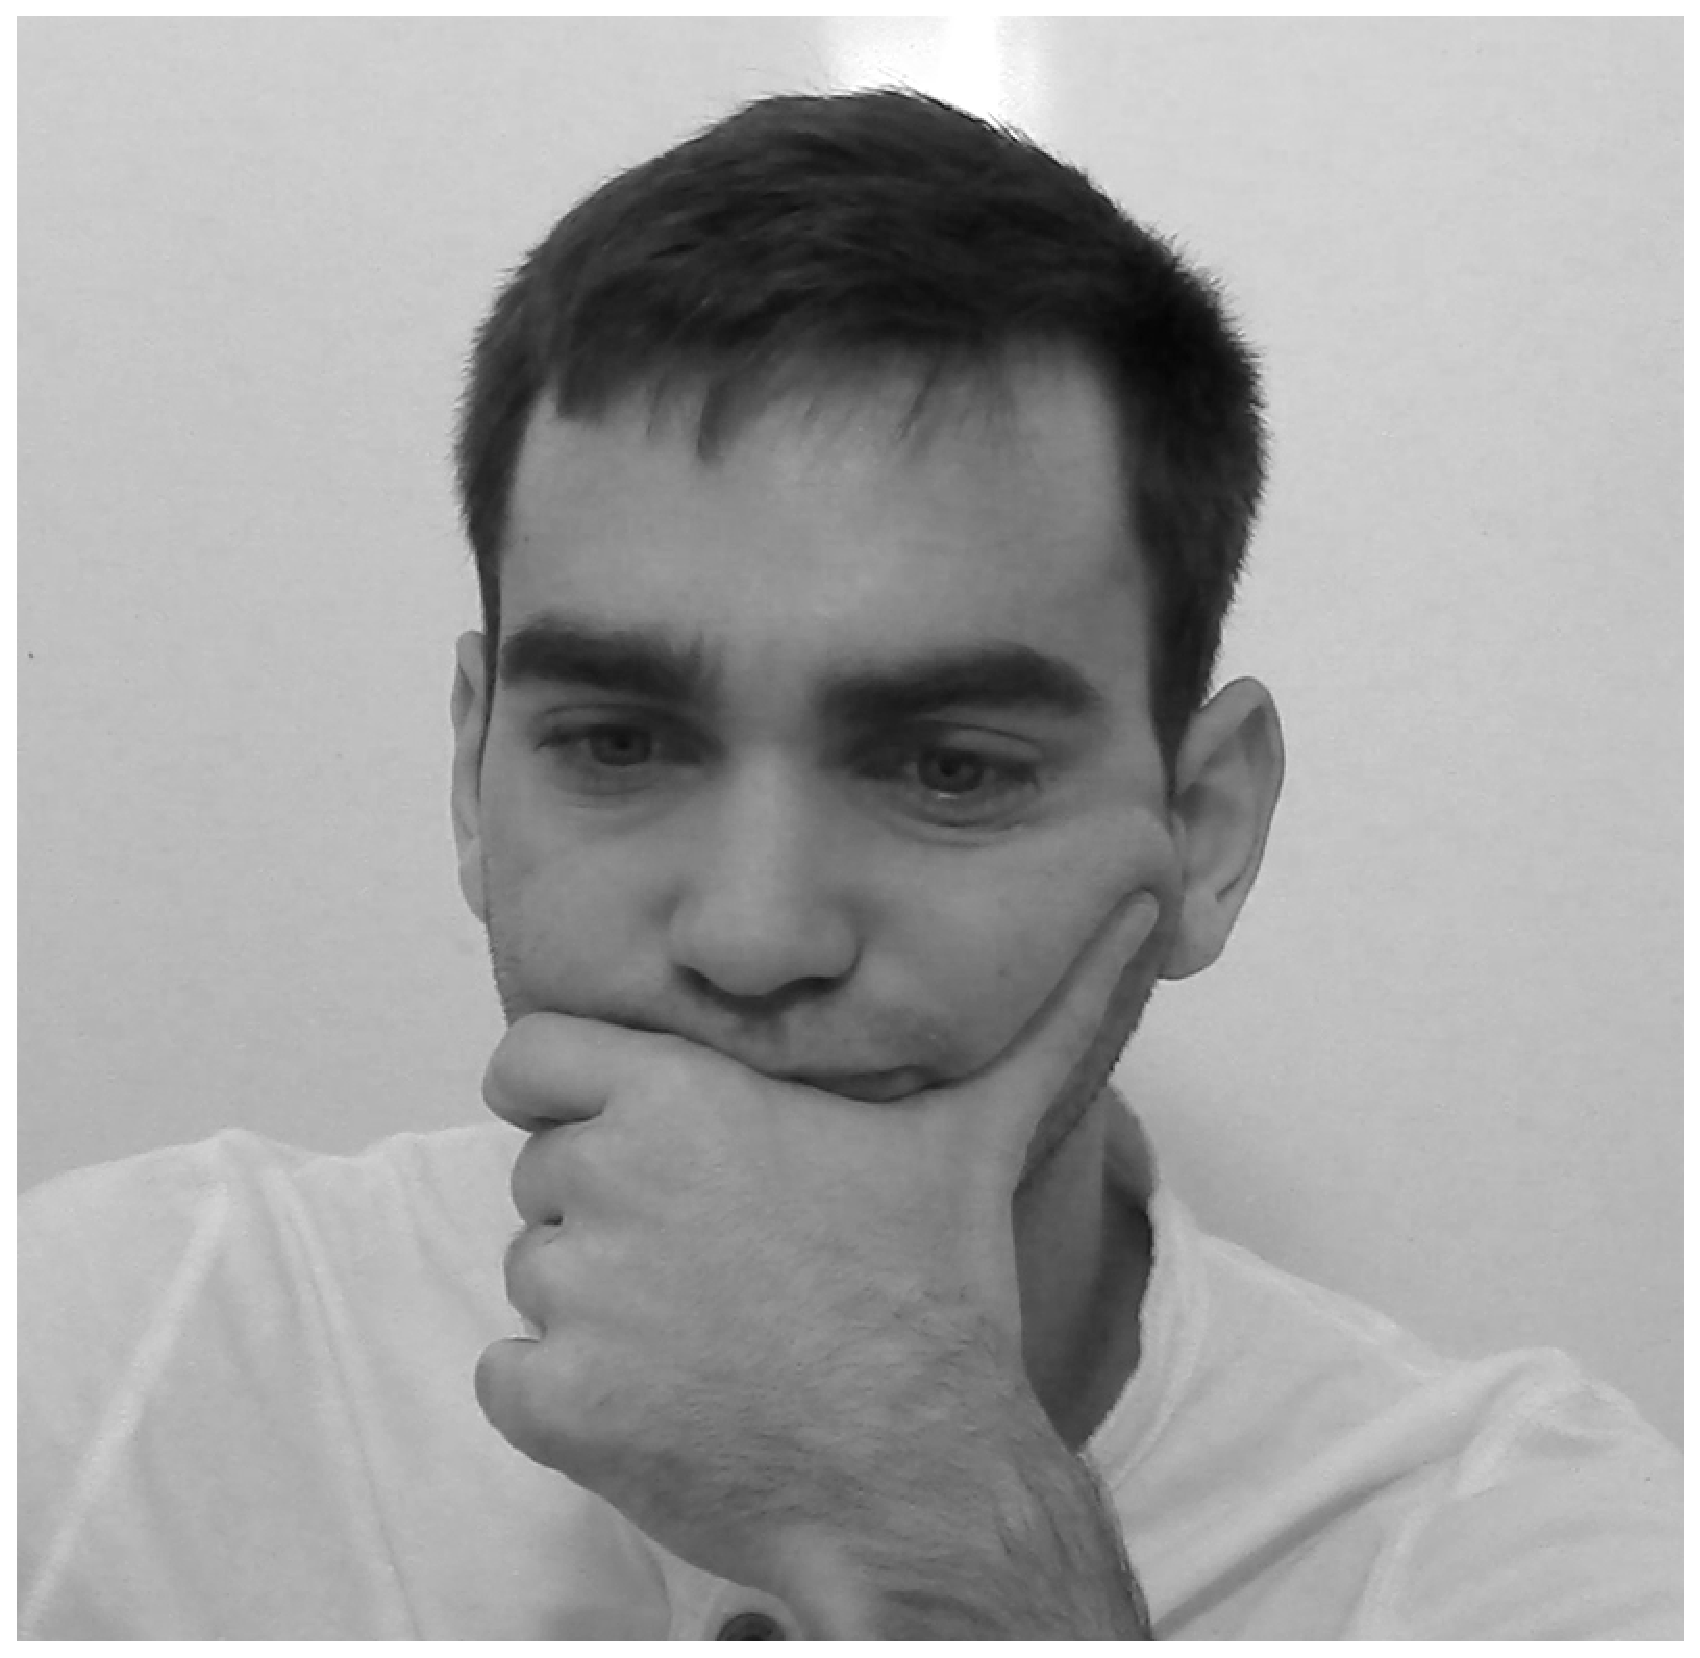
\includegraphics[width=0.95\textwidth]{Content/figures/face-occlusion}
    \caption{}
    \label{fig:face-occlusion}
  \end{subfigure}%
  \begin{subfigure}[b]{0.5\textwidth}
    \centering
    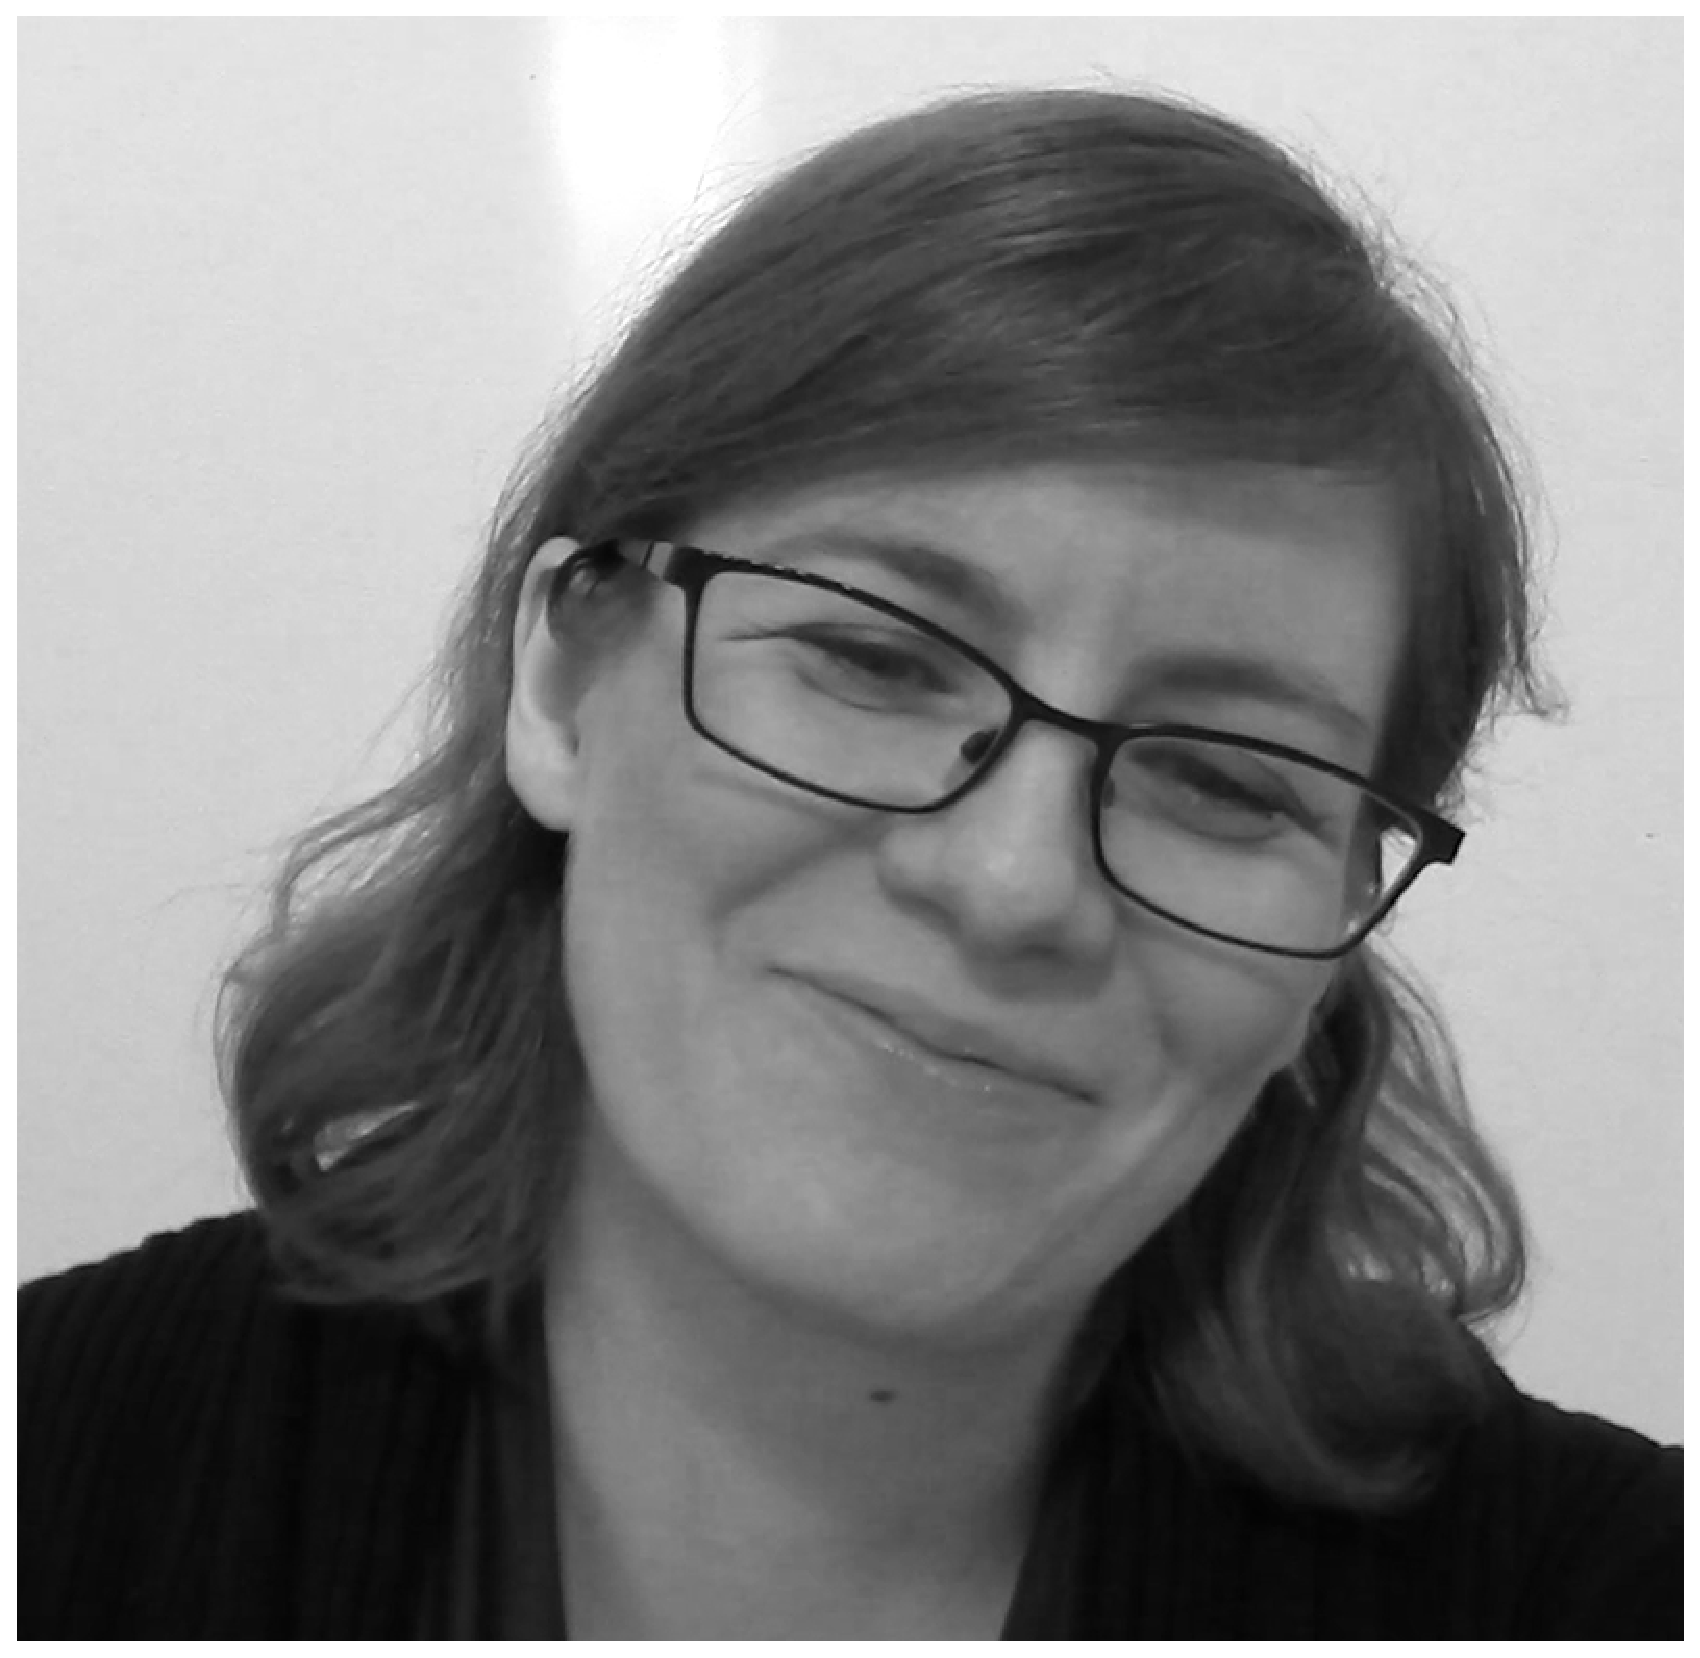
\includegraphics[width=0.95\textwidth]{Content/figures/head-tilt}
    \caption{}
    \label{fig:head-tilt}
  \end{subfigure}
  \caption{Examples of body movement and facial activity during gaming sessions. (a) Partial face occlusion by subject's hand; (b) Head tilt and movement during laugh action.}
  \label{fig:face-variation}
\end{figure}

It is possible to speculate that the variations regarding movement and size of the ROI, which directly influence estimation accuracy of the rPPG technique, seem to be connected to the unique behavior of each user as well. As illustrated by Figures \ref{fig:chart-roi-anomalies-center} and \ref{fig:chart-roi-anomalies-diagonal}, subjects present different movement patterns. Previous analysis of the videos indicates significant differences regarding facial activities among subjects \parencite{bevilacqua2016variations}. It strengthens the idea of a user-tailored model able to deal with such peculiarities, which is more likely to produce better estimations. A method that operates its estimations based on the average user behavior is prone to be significantly affected by specific user behavior outside the expected mean pattern, causing skewed distribution of estimation errors such as the ones presented on Figure \ref{fig:chart-hists} regarding $M_{eRate}$ and RMSE.

%\subsection{Limitations}

%Some limitations of the experimental procedure and analysis should be noted. The 1-minute long duration of each video segment used for the estimation of HR may affect the results. The ideal length of the video segment used for estimation (called window size) is not agreed upon in the literature \parencite{rouast2016remote}. In general, it depends on the characteristics of the rPPG technique being applied as well as the hardware configuration, such as camera framerate \parencite{roald2013estimation}. We selected a 1 min analysis window based on the information of the original work by \textcite{poh2011advancements}. Additionally our experimental procedure consists of games whose difficulty level changes every 1 minute, so that value is aligned with the window size used for HR estimation. As previously described, the statistical nature of ICA, part of the selected rPPG employed in the experiment, demands longer video samples to produce accurate results. The longer the video, however, the higher the chances of subject motion, which increases noise. A trade-off between the duration of the video segments and the estimation accuracy could be better investigated. Our experimental setup used an external light source to minimize noise caused by changes in illumination, which should narrow the estimation error to causes as subject movement and/or facial activity. It is likely, however, that other factors might impact the estimation accuracy, such as facial hair, e.g. beard and hair over the forehead area, use of glasses, and skin color.

\subsection{Conclusions}

Overall the estimation of the rPPG was feasible, showing mean estimation error of 2.99 bpm (SD 18.83 bpm), RMSE of 19.03 bpm and a positive and medium strength Pearson correlation of $r=0.43$, $p < 0.001$. On average, the estimation error of the rPPG technique was up to 10.31\% of the expected value calculated from ground truth. Additionally the exploratory investigation regarding factors that impacted the accuracy of the rPPG technique, such as variations in the region of interest (ROI) used to remotely extract the HR signal, suggest factors connected to the type of the game being played and the unique behavior of each subject influenced the estimations. Among the causes of such influence were identified body movement, e.g. head tilt and rotation, and facial occlusion by subjects hand.
